\documentclass[letterpaper]{article}

%%%%%%%%%%%%%%%%%%%%%%%%%%%%%%%%%%%%%%%%%%%%%%%%%
%%%%                  HI!                    %%%%
%%%%        THIS IS THE SSI-BIOLOGY			 %%%%
%%%%      GENERIC PROCEDURE TEMPLATE :) 	 %%%%
%%%%      IT MIGHT LOOK SCARY, BUT IT'S 	 %%%%
%%%%           PRETTY EASY TO USE 			 %%%%
%%%%%%%%%%%%%%%%%%%%%%%%%%%%%%%%%%%%%%%%%%%%%%%%%

%%%%%%%%%%%%%%%%%%%%%%%%%%%%%%%%%%%%%%%%%%%%%%%%%%%%%%%%%%
%%%%      RIGHT NOW YOU'RE LOOKING AT BOILERPLATE     %%%%
%%%%  THAT IS, THINGS YOU DON'T HAVE TO CHANGE (EVER) %%%%
%%%%     SCROLL DOWN FOR THE THINGS YOU SHOULD PAY    %%%%
%%%%    ATTENTION TO :)  (YOU'LL KNOW WHEN TO STOP)   %%%%
%%%%%%%%%%%%%%%%%%%%%%%%%%%%%%%%%%%%%%%%%%%%%%%%%%%%%%%%%%


%% Language and font encodings
\usepackage[english]{babel}
\usepackage[utf8x]{inputenc}
\usepackage[T1]{fontenc}

%% Sets page size, footer, indent and margins
\usepackage[a4paper,top=2.5cm,bottom=2.5cm,left=2.25cm,right=2.25cm,marginparwidth=2.25cm]{geometry}
\setlength\parindent{0pt}
\setlength{\footskip}{55pt}

%% Useful packages
\usepackage{amsmath}
\usepackage{graphicx}
\usepackage{fancyhdr}
\pagestyle{fancy}
\usepackage{textcomp}
\usepackage{gensymb}
\usepackage{hyperref}
\usepackage{readarray}
\usepackage{verbatimbox}
\usepackage{framed}
\usepackage[dvipsnames]{xcolor}
\usepackage{tcolorbox}
\usepackage{colortbl}
\usepackage{libertine} 
\usepackage{siunitx}
\usepackage{wrapfig}

% Safety Environment 
\definecolor{safetyFrame}{HTML}{FFFFFF}
\newenvironment{safety}{%
\begin{tcolorbox}[width=\textwidth, colframe=safetyFrame, arc=1.5mm]
}%
{\end{tcolorbox}}


% Footer
\lfoot{
\includegraphics[height=1.5cm]{1000x350-Horiz-Logo-WhiteRed-BlackText.png}}
\rfoot{
\includegraphics[height=1.25cm]{smol.png}}

% Substitution Commands
\newcommand{\tdt}{Terminal Deoxynucleotidyl Transferase}
\newcommand{\C}{\degree{}C}
\newcommand{\uL}{\micro{}L}
\newcommand{\BdATP}{3'-O-(2-nitrobenzyl)-2'-dATP}

%Custom Commands
\newcommand{\B}[1]{\textbf{#1}}

% Safety Info
\newcommand{\SYBRGOLD}{\item{\B{SYBR Gold} has no data available addressing the mutagenicity or toxicity of SYBR® Gold nucleic acid gel stain. Because this reagent binds to nucleic acids, it should be treated as a potential mutagen and handled with appropriate care. The DMSO stock solution should be handled with particular caution as DMSO is known to facilitate the entry of organic molecules into tissues.\cite{sybrGold}}}
\newcommand{\SYBRI}{\item{\B{SYBR Green I} is a mutagen and can penetrate laboratory gloves in a relatively short period of time, please change your gloves in the event of contamination. See \url{http://www.sigmaaldrich.com/MSDS/MSDS/DisplayMSDSPage.do?country=US&language=en&productNumber=S9430&brand=SIAL} for more information on the specifics of SYBR Green I. 
}}
\newcommand{\ETBR}{\item{\B{Ethidium Bromide} is a \B{serious mutagen} and is \B{significantly carcinogenic}. If working with considerable amounts, a \B{fume hood and respirator} are warranted. For more information see \url{https://www.sciencelab.com/msds.php?msdsId=9927667}
}}


% Shortcuts

%Stop Point (Optional)
\newcommand{\stopPoint}{\begin{center}
\rule{0.5\textwidth}{.4pt}\\
\vspace{1mm} 
OPTIONAL STOP POINT\\
\rule{0.5\textwidth}{.4pt}
\end{center}}

\newcommand{\RstopPoint}{\begin{center}
\rule{0.5\textwidth}{.4pt}\\
\vspace{1mm} 
RECOMMENEDED STOP POINT\\
\rule{0.5\textwidth}{.4pt}
\end{center}}

% Dilution Macro
\newcommand{\Dilution}[4]{
\subsection{#2}
\begin{enumerate}
\item{Vortex #2 stock}
\item{Pipette #1\uL{} #2 into a PCR Tube}
\item{Pipette #3\uL{} #4 into solution}
\item{Vortex until mixed}
%\item{Pipette $#2\mu L$ Water into solution}
\end{enumerate}
}

% Gel Macro
\newcommand{\gel}[4]{
\begin{figure}[ht]
\label{#2}
\begin{center}
\includegraphics[width=0.45\textwidth]{#1}
\caption{#2}
\end{center}
\subsection{#3 Analysis}
#4
\end{figure}
}

% Well plate Macro
\newcommand{\wellplate}[2]{
\getargsC{#1}
\begin{tabular}{*{1}{>{\columncolor{blue!20}}l}|l|l|l|l|l|l|l|l|l|l|l|l|}
\rowcolor{blue!20}%
 & 1  & 2  & 3  & 4  & 5  & 6 & 7 & 8 & 9 & 10 & 11 & 12\\ \hline
\ifdefined\argxii
A & \argi & \argii & \argiii & \argiv & \argv & \argvi & \argvii & \argviii & \argix & \argx & \argxi & \argxii \\ \hline\fi
\ifdefined\argxxiv
B & \argxiii & \argxiv & \argxv & \argxvi & \argxvii & \argxviii & \argxix & \argxx & \argxxi & \argxxii & \argxxiii & \argxxiv \\ \hline\fi
\ifdefined\argxxxvi
C & \argxxv & \argxxvi & \argxxvii & \argxxviii & \argxxix & \argxxx & \argxxxi & \argxxxii & \argxxxiii & \argxxxiv & \argxxxv & \argxxxvi \\ \hline\fi
\ifdefined\argxlviii
D & \argxxxvii & \argxxxviii & \argxxxix & \argxl & \argxli & \argxlii & \argxliii & \argxliv & \argxlv & \argxlvi & \argxlvii & \argxlviii \\ \hline\fi
\ifdefined\arglx
E & \argxlix & \argl & \argli & \arglii & \argliii & \argliv & \arglv & \arglvi & \arglvii & \arglviii & \arglix & \arglx \\ \hline\fi
\ifdefined\arglxxii
F & \arglxi & \arglxii & \arglxiii & \arglxiv & \arglxv & \arglxvi & \arglxvii & \arglxviii & \arglxix & \arglxx & \arglxxi & \arglxxii \\ \hline\fi
\ifdefined\arglxxxiv
G & \arglxxiii & \arglxxiv & \arglxxv & \arglxxvi & \arglxxvii & \arglxxviii & \arglxxix & \arglxxx & \arglxxxi & \arglxxxii & \arglxxxiii & \arglxxxiv \\ \hline\fi
\ifdefined\argxcvi
H & \arglxxxv & \arglxxxvi & \arglxxxvii & \arglxxxviii & \arglxxxix & \argxc & \argxci & \argxcii & \argxciii & \argxciv & \argxcv & \argxcvi \\ \hline\fi
\end{tabular}
}

\newcommand{\tdtSafety}{\item{\textbf{\tdt{}} is toxic if inhaled. May cause cancer. Toxic to aquatic life with long lasting effects. Avoid breathing dust/fume/gas/mist/vapours/spray. Use personal protective equipment as required. If Inhaled: Remove victim to fresh air and keep at rest in a position comfortable for breathing. Dispose of contents/container in accordance with local/regional/national/international regulations.\cite{Invitrogen2002}}}

\usepackage{enumitem,amssymb}
%%%%%%%%%%%%%%%%%%%%%%%%%%%%%%%%%%%%%%%%%%%%%%%
%%%%%%%%%%%%%%%%%%%%%%%%%%%%%%%%%%%%%%%%%%%%%%%
%%%%%%%%%%%%% End of Boiler Plate %%%%%%%%%%%%%
%%%%%%%%%%%%%%%%%%%%%%%%%%%%%%%%%%%%%%%%%%%%%%%
%%%%%%%%%%%%%%%%%%%%%%%%%%%%%%%%%%%%%%%%%%%%%%%

%%%%%%%%%%%%%%%%%%%%%%%%%%%%%%%%%%%%%%%%%%%%%%%
%%%%%   AKA YOU WRITE AFTER THIS POINT    %%%%%
%%%%%%%%%%%%%%%%%%%%%%%%%%%%%%%%%%%%%%%%%%%%%%%


\title{\BdATP{} Incorporation Detection with PAGE Assisted Precision Version 3} % CHANGE THIS
\author{Written by \textbf{Michael Uttmark}\\ % CHANGE THIS 
		Not Peer Reviewed\\%Checked by \textbf{}\\ % CHANGE THIS
        For the Stanford Student Space Initiative Biology Subteam}
\date{\textbf{Written:} October 9, 2017 \,\textbf{Preformed:} October 12, 2017 \,\textbf{Printed:} \today{}}

\begin{document}

\maketitle
\section{Procedure Purpose} % CHANGE THIS
Determine if the the modified nucleotide, \BdATP{}, can be noticeably incorporated by \tdt{} in "standard conditions" while determining the blocking efficacy \& purity of our \BdATP{} stock.
\begin{figure}[ht]
\centering
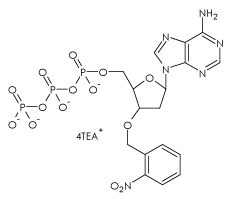
\includegraphics[width=2in]{1.png}
\caption{\BdATP{}}
\label{bdatp}
\end{figure}
\section{Overview} % CHANGE THIS 
This lab will attempt to append \BdATP{} to a \textbf{very short (5bp) primer}. The effectiveness of this attempt will be determined by attempting to form a homopolymer on the modified primer. If a homopolymer is formed, the blocking groups did not effectively prevent their formation. This could be due to many reasons (the most likely of which being that the blocking groups either (1) were appended without the 2' nitrobenzyl due to sample degradation or (2) were not appended). If the homopolymer was not formed (but a homopolymer was formed on the controls) it follows that the blocking groups prevented the formation of the homopolymer, likely due to them preforming their intended function. Moreover, all samples will be run on a PAGE gel in order to achieve single nucleotide resolution. This will allow us to confirm that the \BdATP{} is the only base appended to the "blocked" sample. A ddATP control will help as well.

% Safety First! ALSO, % CHANGE THIS
\section{Safety Information}
\begin{safety}
\begin{enumerate}
\SYBRGOLD{} % For select reagents, I've created custom commands so we don't have to copy and paste every time :)
\tdtSafety{}
\item{Working in a communal lab space is dangerous. Do not assume your fellow workers cleaned up sufficiently}
\end{enumerate}
\end{safety}

\section{Materials}
\begin{itemize}
\item{Primer: TCATC}
\item{100mM \BdATP{} Stock}
\item{100mM dNTP Stock}
\item{100mM dATP Stock}
\item{10mM ddATP Stock}
\item{5X \tdt{} Buffer}
\item{\tdt{} Stock (20U/\uL{})}
\textbf{Note:} Only one stock solution is at 20U/\uL{}, \textbf{be sure you have the right one.}
\item{Nuclease Free Water}
\item{TBE Buffer}
\item{15\% Urea Denaturing Gels}
\item{SYBR Gold}
\end{itemize}
% Now for the _good_ stuff  

\textbf{Note}: If the bioanalyzer is a valid analysis method, make a "copy" of PCR Tube B. Then store the second B as per the Stop Procedure after completion of step 13. This $\rightarrow\,\square\,$ will be checked if the second B should be made.
\section{Procedure}% CHANGE THIS
\begin{enumerate} 
\subsection{Sample Preparation}
\item{Remove \BdATP{}, \tdt{}, primer, \tdt{}  buffer, ddATP stock and dATP stock from -20\C{} freezer}
\item{Let \BdATP{} thaw on ice in dark}
\item{Other reagents can thaw on ice in the light}
\subsection{Attempted blocking}
\item{Label three PCR Tubes A, B and D, respectively}
\item{Pipette 10\uL{} of nuclease free water into both PCR Tubes}
\item{Pipette 4.0\uL{} 5X \tdt{} reaction buffer into both PCR Tubes}
\item{Dilute Nucleotides:
\begin{enumerate}
\item{Label a PCR Tube "dATP Dilute"}
\item{Pipette 9\uL{} of nuclease free water into PCR Tube}
\item{Pipette 1\uL{} of dATP stock into PCR Tube}
\item{Vortex directly before use}
\end{enumerate}
NOTE: This step can be skipped, as this dilute has already been made. The dilution instructions are redundant, and are here in case we want to repeat the experiment in the future.
\begin{enumerate}
\item{Label a PCR Tube "\textbf{BdATP} Dilute" (make this \textit{very} clear)}
\item{Pipette 9\uL{} of nuclease free water into PCR Tube}
\item{Pipette 1\uL{} of \BdATP{} stock into PCR Tube}
\item{Keep in \textbf{dark} and vortex directly before use}
\end{enumerate}
}
\item{Pipette .5\uL{} of primer into all three PCR Tubes}
\item{Pipette 2\uL{} of dATP dilute into PCR Tube A}
\item{Pipette 2\uL{} of \BdATP{} dilute into PCR Tube B}
\item{Pipette 2\uL{} of ddATP \textbf{10mM stock} into PCR Tube D}
\item{Gently pipette 1.5\uL{} \tdt{} (\textbf{20 U/\uL{}}) into all three PCR Tubes}
\item{Incubate sample at 37\C{} for 30 minutes}\\
Note: \textbf{Do NOT} deactivate \tdt{} 
\stopPoint{} 
\subsection{Extending}
Based off of our standard \tdt{} extending procedure \cite{genTdT}.
\item{Label two PCR Tubes C and X, respectively}
\item{Pipette 10\uL{} nuclease free water into PCR Tube C (see above, \textbf{ATTEMPTED BLOCKING})}
\item{Pipette 10\uL{} of nuclease free water into PCR Tube X (see above, \textbf{CONTROLS})}
\item{Pipette .5\uL{} of primer into both PCR Tubes}
\item{Set PCR Tube X aside.}
\item{Pipette 4.0\uL{} 5X \tdt{} reaction buffer into PCR Tube C}
\item{Pipette .6\uL{} of dNTP stock into PCR Tube \textbf{C}}
\item{Pipette .4\uL{} of dNTP stock into PCR Tubes \textbf{A, B}}
\item{Gently pipette 1.5\uL{} \tdt{} (20 U/\uL{}) into \textbf{PCR Tube C} (note, this is not from the standard 15U\uL{} stock)}
\item{Incubate \textbf{all} samples at 37\C{} for 30 minutes}\\
\RstopPoint{} 
\subsection{Analysis}

\subsubsection{Prepare Gel}
\item{Prepare a 15\% Denaturing Urea-PAGE gel.}\\
Note: PAGE Gels are stored in the cold room. If 15\% PAGE gels are not available, use 20\% denaturing urea PAGE gels as a substitute.
\begin{enumerate}
\item{Do not invert the gel at any point.}
\item{Get help from Cynthia, Lillian or Alan if possible. If uncomfortable, freeze samples.}
\item{Remove clip from gel with special tool. If tool is not available, be very careful.}
\item{After the gel and it's associated apparatus and buffers have been situated, rinse each well with 15 uL of .5X TBE buffer.}
\end{enumerate}
\item{Allow to pre-run at 200V for 20 minutes prior to continuing.}

\subsubsection{Run Gel}
NOTE: Ensure that the loading dye has Bromophenol Blue in it.
\item{Add 8\uL of samples A, B, D, C and X with 1.5\uL{} of loading dye for a total volume of 8\uL to gel respectively, left to right with the wells at the top.}
\item{Add 10\uL{} of Loading Dye to the well twice to the right of X (the seventh well from the left).}
\item{Add an appropriate amount of ladder (annotate the amount added on this sheet) the the far right well (wells at the top).}
\item{Add a 50/50 combination of sample \textbf{B} and sample \textbf{C} to the sixth well. That is, add \textbf{3\uL{}} of sample \textbf{B}, \textbf{3\uL{}} of sample \textbf{B} and \textbf{1.2}\uL{} of loading dye to the sixth well, from the left with the wells at the top.}
\item{Run at 200V}
\item{Remove gel once the Bromophenol Blue has almost reached the $\frac{3}{4}$ point \cite{dnaAgarose}}

\subsubsection{Stain \& View Gel}
\item{While the gel runs, prepare 1X SYBR Gold Staining Solution with TBE as dilute}
\item{Once gel has finished running, \textbf{\textit{lightly}} agitate gel while submerged in solution for 40 minutes.}
\item{Review gel with gel viewer. Until unnecessary, place gel back in stain for 20 minute increments and re-image.}
\item{Post pictures to Slack.}\\
\end{enumerate} 

% Stop Procedure
\section*{Stop Procedure}
\begin{enumerate}
\item{Pipette samples into PCR tubes if not already contained in an appropriate manner}
\item{Label containers if not already labeled}
\item{Freeze samples at -20\C{}}
\end{enumerate}

\section{Result Analysis}
\subsection{Summary}

\subsection{Gel Analysis}

\begin{figure}[ht]
\label{Hybrid Gel}
\begin{center}
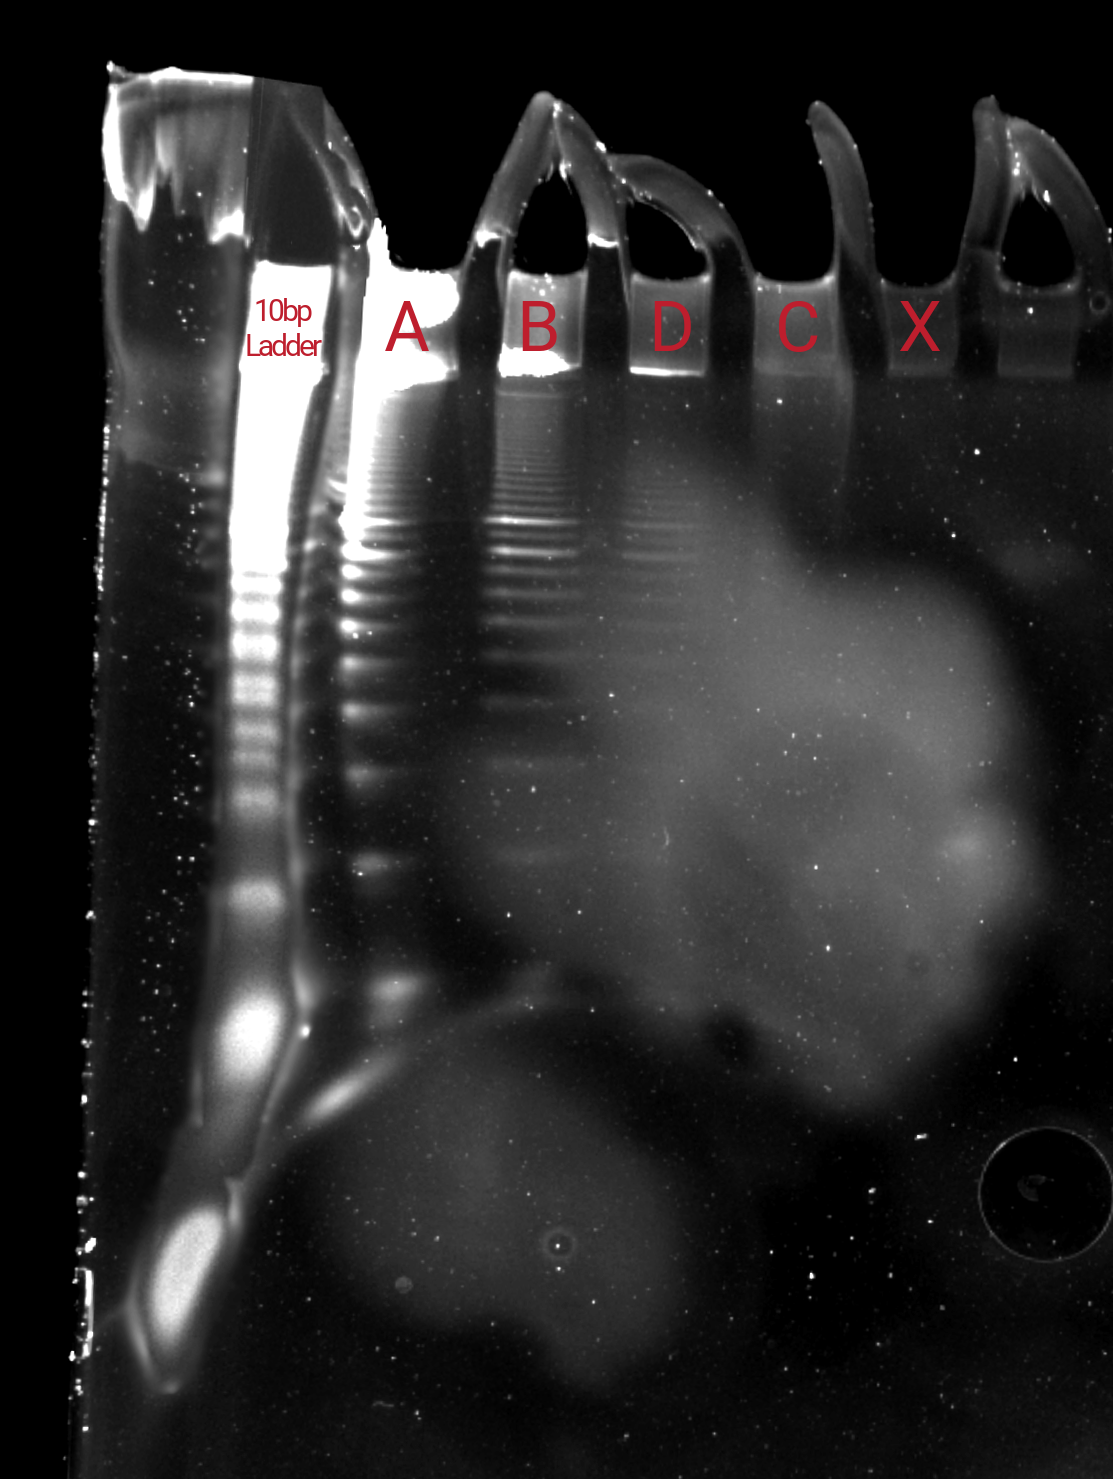
\includegraphics[width=0.45\textwidth]{./gels/composite-gel-cropped.png}
\caption{Digital Combination of PAGE gels from the Third Run of this experiment}
\end{center}
\subsection{Hybrid Gel Analysis}
\end{figure}
\begin{wrapfigure}{r}{0.15\textwidth}
\centering
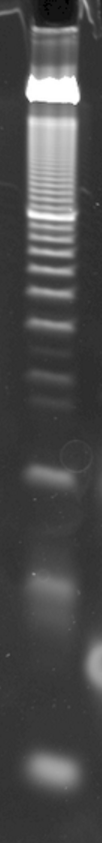
\includegraphics[height=1.5in]{ladder-ideal.png}
\caption{Ideal Ladder}
\label{Ideal Ladder}
\end{wrapfigure}
This "gel" is a digital combination of multiple exposure lengths. The gels were combined to increase the visibility of our "samples". The gels are pictured unedited below in Figures \ref{gels3} \& \ref{gels2}.

From left to right, we \textit{should} have a ThermoFisher 10bp  Ladder, samples A, B, D, C and X. The lane to the right X had 5\uL{} of loading dye in it. However, judging from the results, this is \textbf{not} an accurate description of the actual contents of the gel. Before we discuss our hypothesis for what went wrong, let us address what ideally \textit{should} have happened.

In lane 1 (numbering left to right) we should have seen a ladder resembling the ladder to the right in Figure \ref{Ideal Ladder}. Figure \ref{Ideal Ladder} depicts the same 10bp ladder from ThermoFisher on and identical gel. Moreover, it was run via the same protocol as our "Perfect Page III" that this procedure's gel based analysis section was modeled after. The main differences between this procedure and that of Perfect Page III (other than the DNA being analyzed) is the amount of ladder added. In this procedure, we added 1\uL{} of stock while in Perfect Page III only 0.5\uL{} was added. This was done because the 0.5\uL{} added in the initial agarose based \BdATP{} Incorporation Detection resulted in a ladder that was too weak after 40 minutes of staining. Our concentrations of DNA were between the second and third dilutions of Perfect Page III, both of which appeared satisfactorily. As such, \textit{given that there was no human error} the result above should not have resulted.\\

In row A, we should have seen a smear characteristic of a standard \tdt{} extension. Whether or not this smear is present isn't clear from the images collected.\\ 

In row B, we should have seen a 6bp oligo due to the addition of a \BdATP{} to our initial 5bp primer. These predicted results are not visually present in the images we collected. Nor, however, is the smear characteristic of a standard \tdt{} extension that would have appeared had there been an issue with the performance of the \BdATP{}.\\

In row D we should have 6bp oligo due to the addition of a dideoxyadenosine triphosphate to our initial 5bp primer (similar to row C). These predicted results are not visually present in the images we collected. Nor, however, is the smear characteristic of a standard \tdt{} extension that would have appeared had there been an issue with the performance of the dideoxyadenosine triphosphate.\\

In row C, we should have seen a smear characteristic of a standard \tdt{} extension. Whether or not this smear is present isn't immediately clear from the images we collected, but there does seem to be some smearing (see Figure \ref{Hybrid Gel}).

\begin{wrapfigure}{r}{0.25\textwidth}
\centering
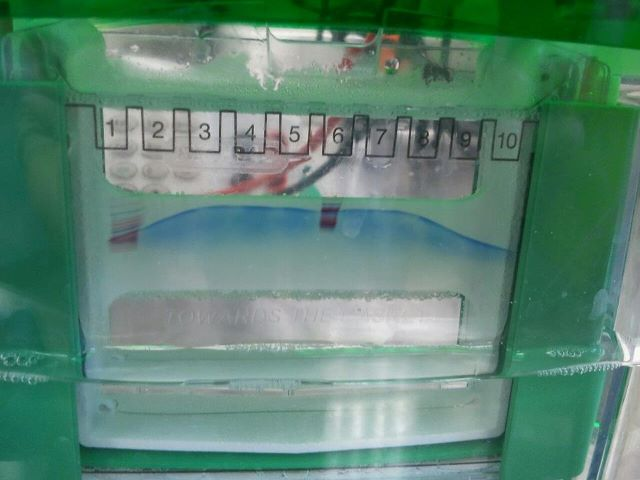
\includegraphics[height=1in]{smiling.png}
\caption{Upside-down Smile on SDS-PAGE Gel{\small (via ResearchGate)}}
\label{Upside-down Smile}
\end{wrapfigure}

In row X, we should have seen a 5bp oligo. This was the only reagent present in the sample. Again, this is not visually present in the images we collected.\\

We also should have seen an even travel of the samples. We did not. What we did see was a "upside down smile" like depicted in Figure \ref{Upside-down Smile}. This is likely due to (1) too much current (and by relation, too much voltage) (which was never noticed in Perfect Page I, Perfect Page II, or Perfect Page III) or (2) the gel was not pressed securely against the gaskets which allowed buffer to leak out\cite{smileSDS}. It seems that the gel was not pressed securely against the gaskets, as we did not see similar behavior in Perfect Page I, Perfect Page II, or Perfect Page III. 

The question remains: why is there ladder in the rows, A, B and D? And why does the intensity of the ladder decrease as the rows get farther and father away from the ladder row? I propose a two fold explanation: First, the ladder was prepared at too high of a concentration. This prediction rests on the fact that the ladder is much \textit{much} brighter when imaged than we expected. Secondly, when the ladder was pipetted into row 1, a small amount of ladder was present on the \textit{outside} of the pipette tip. When the tip entered the buffer, it fell from the tip into wells A, B and D. Moreover, the motion of the tip from left to right would have created a fluid motion conducive to more DNA ending up in the well of A rather than the well of D. Given that the ladder was sufficiently over concentrated, a single \uL{} present on the tip would be more than enough to result in a gel like Figure \ref{Hybrid Gel}. This could have been prevented by (1) preparing the ladder correctly and (2) being \textit{extra} careful when pipetting samples into the SDS-PAGE gel. This is the most convincing hypothesis of error yet. It also implied that our sample is in the gel, we just can't see it. It also means that \textit{no scientifically sound conclusions} regarding \BdATP{} and it's efficiency of incorporation can be made from the images collected in this experiment.

\begin{figure}[ht]
\begin{center}

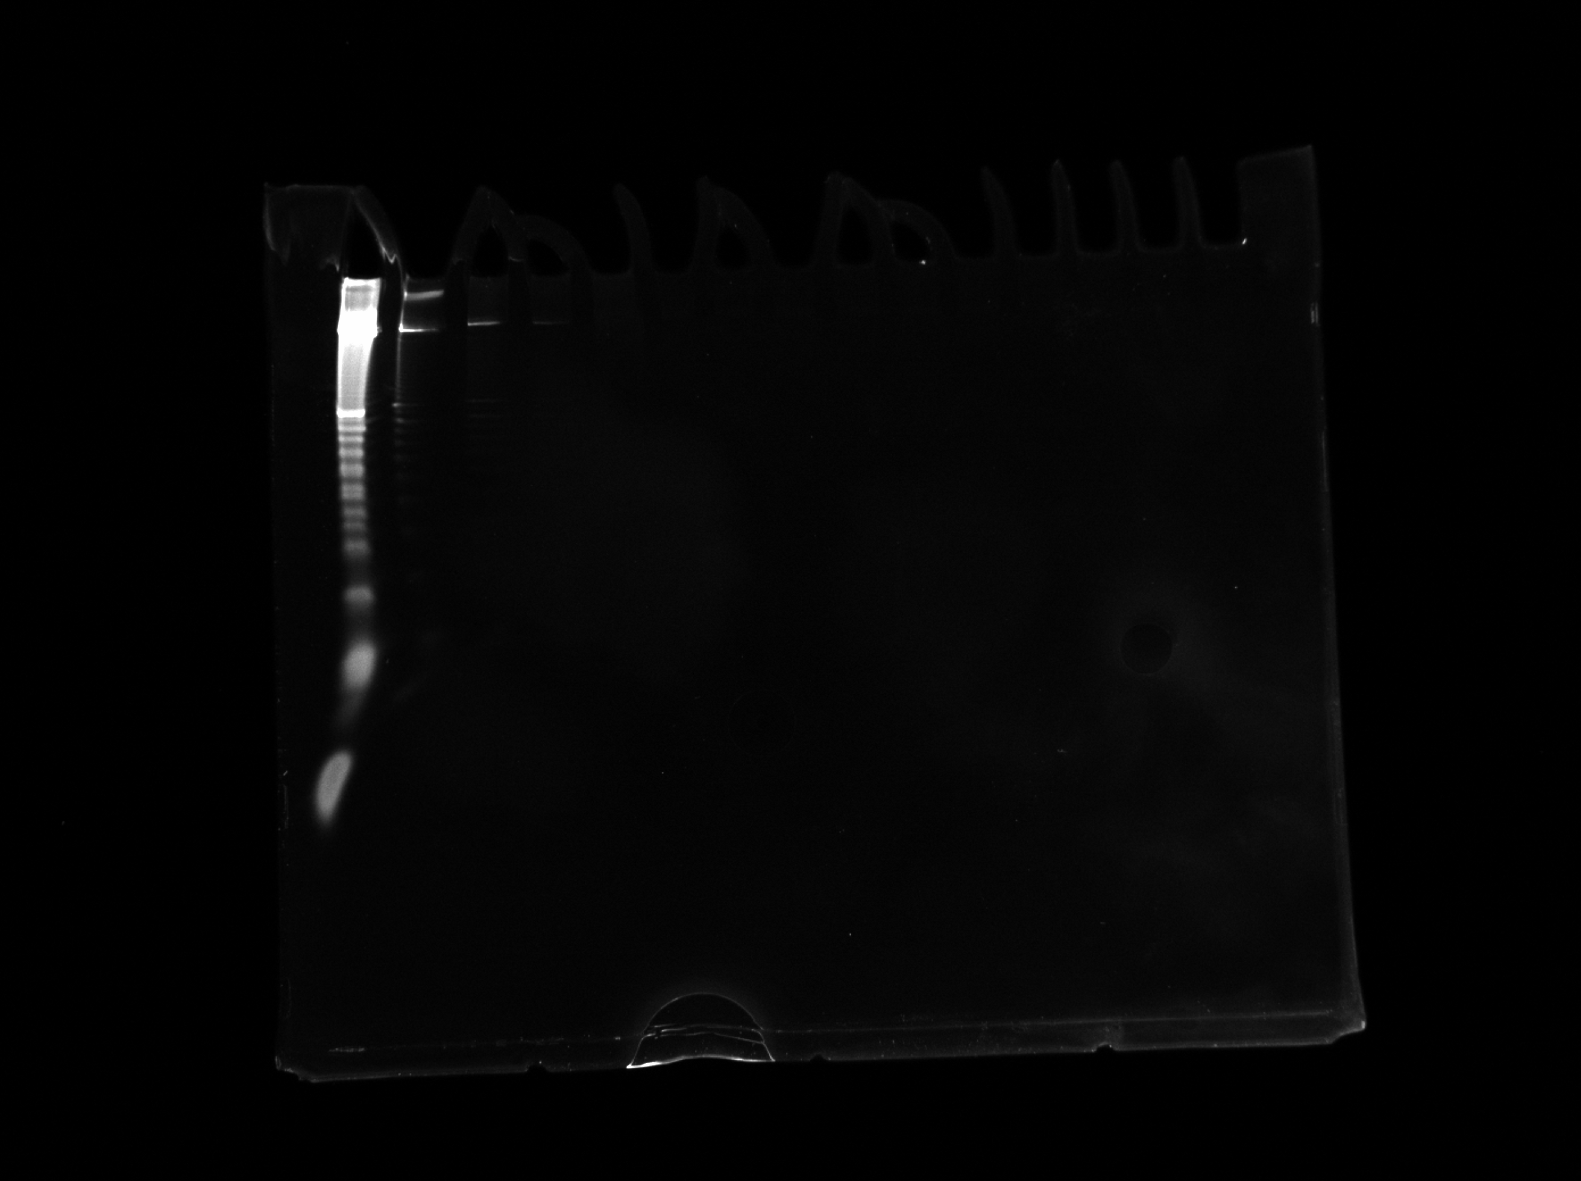
\includegraphics[width=0.3\textwidth]{./gels/under-_05s-small.png}
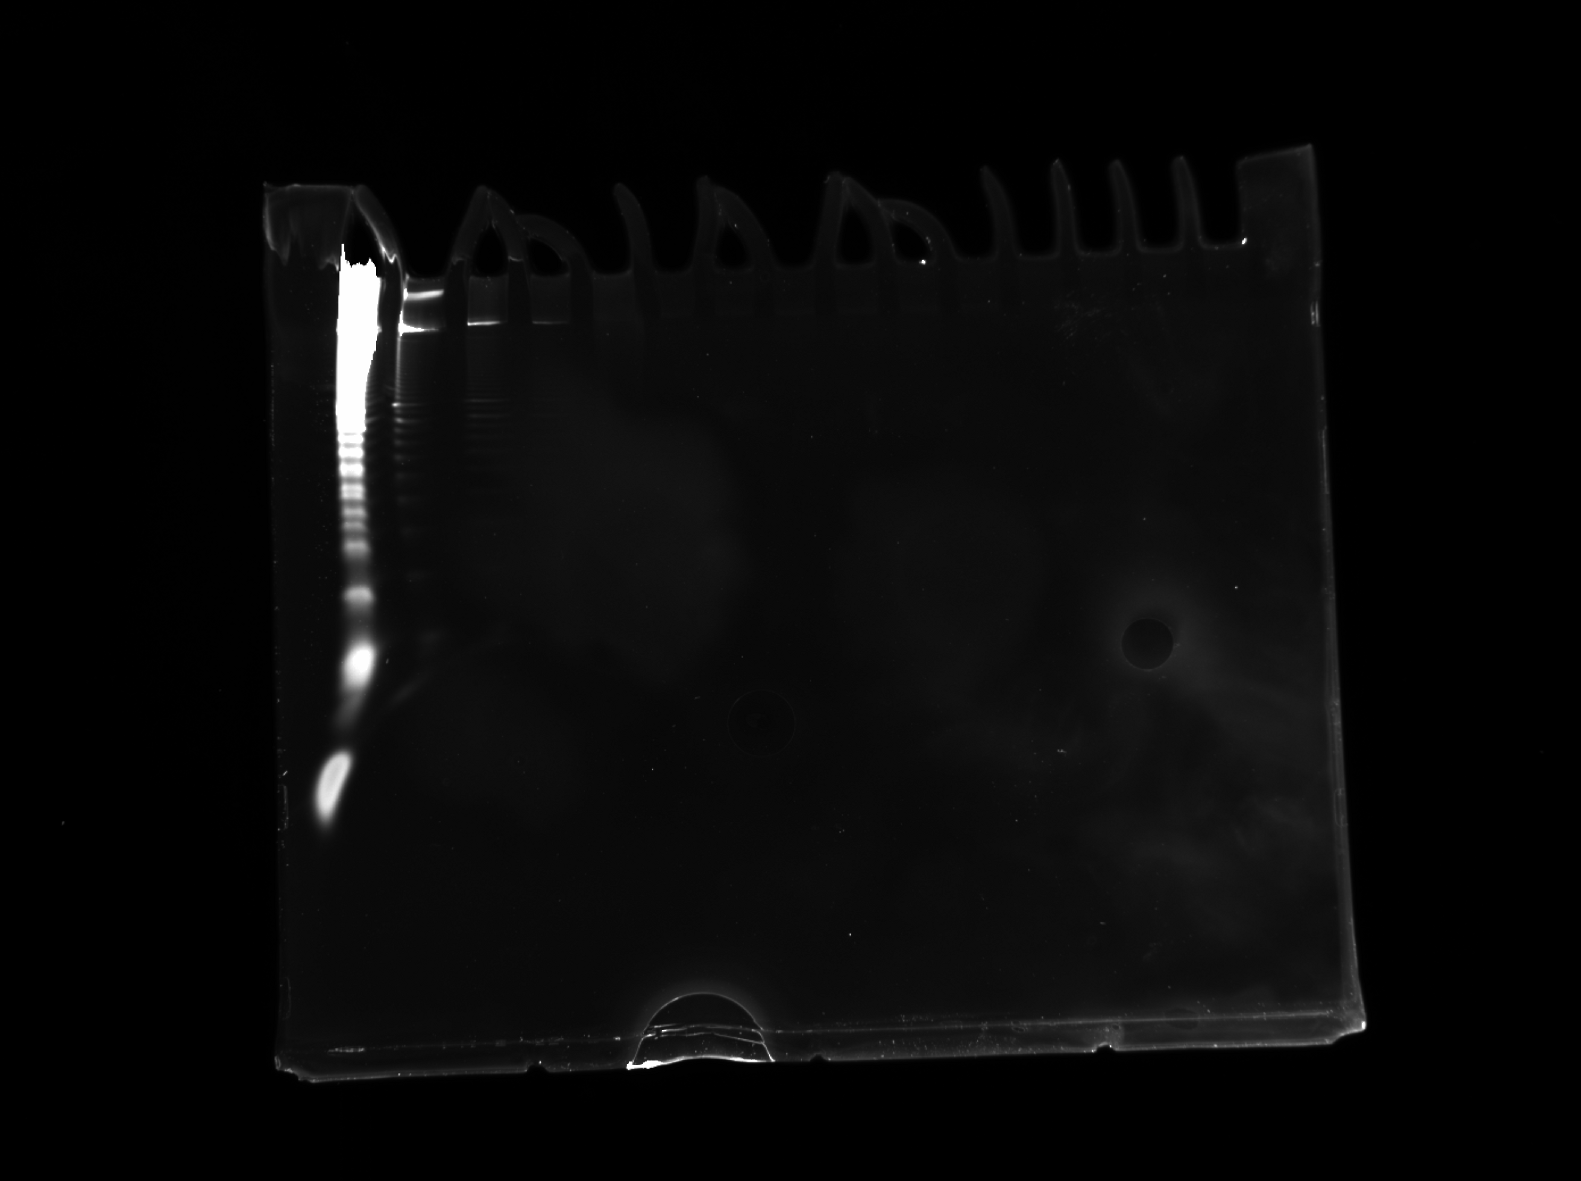
\includegraphics[width=0.3\textwidth]{./gels/faintbands-small.png}
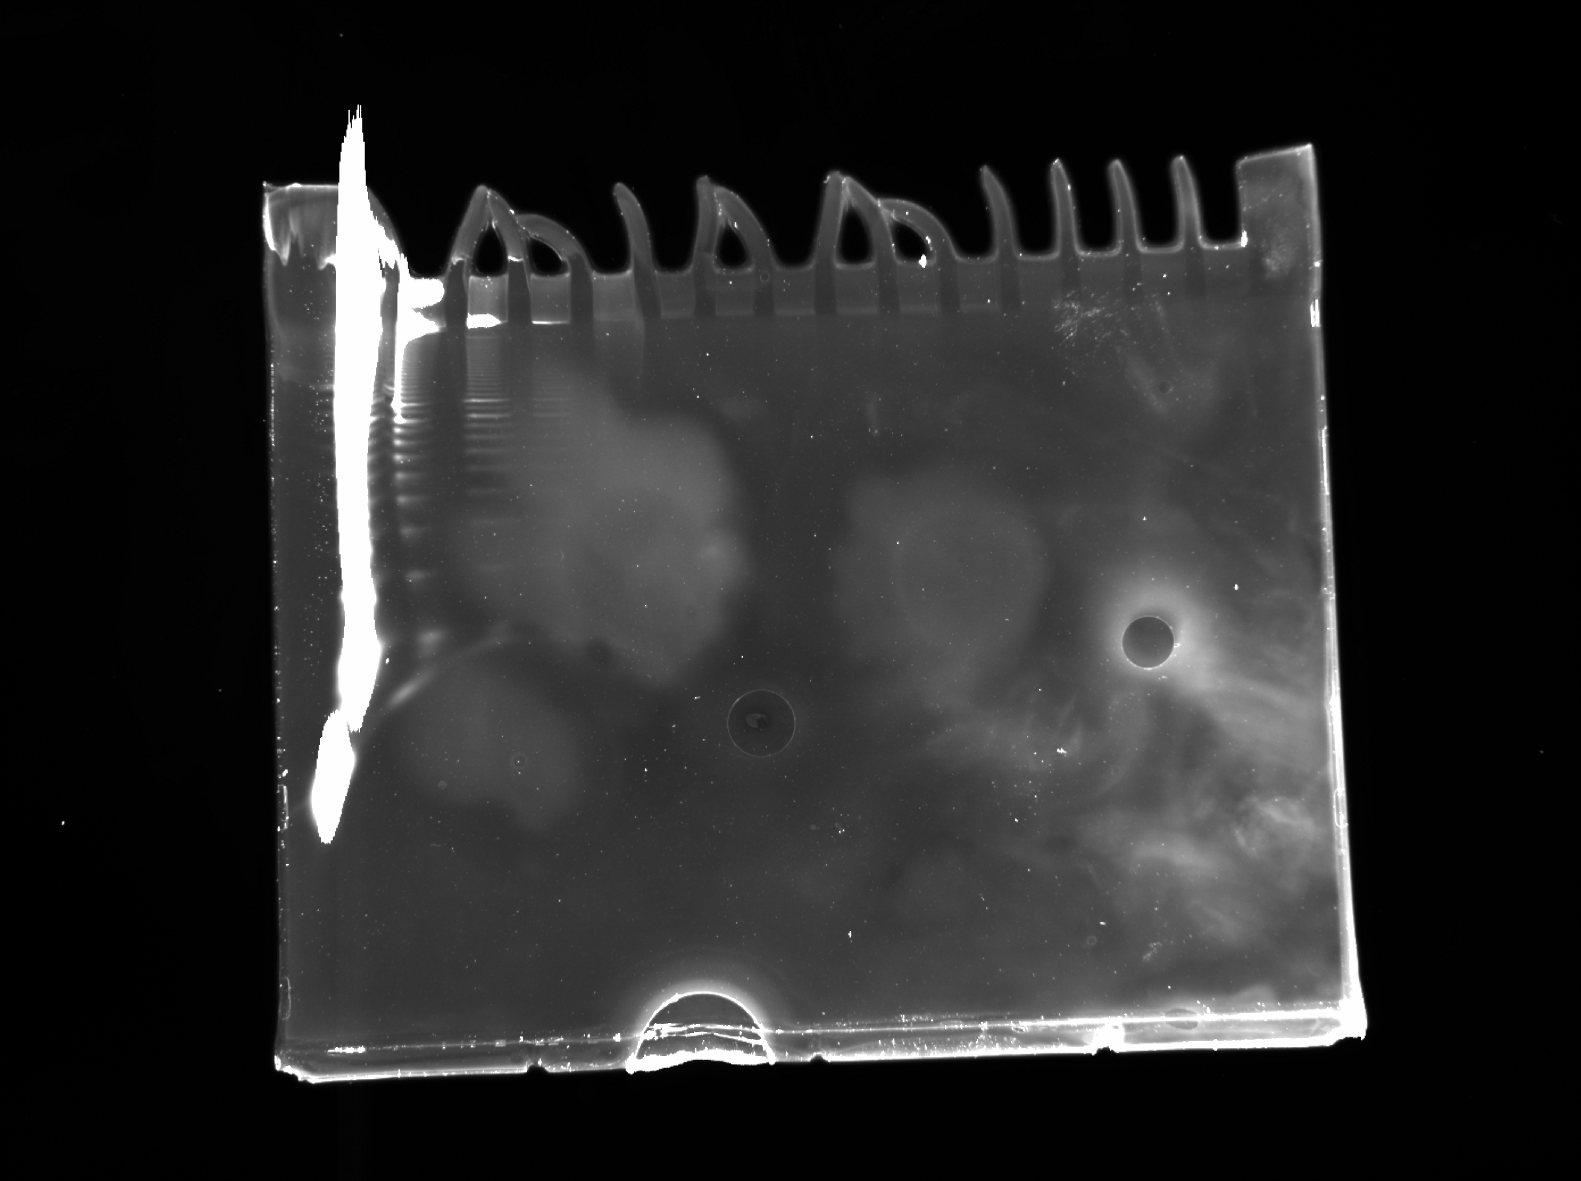
\includegraphics[width=0.3\textwidth]{./gels/over-5s-small.png}

\label{gels3}
\caption{Unedited Gels from Version 3}
From left to right, we have the respective exposure times: 0.1 seconds, faint-band-optimized and 5 seconds.
\end{center}
\end{figure}


\begin{figure}[ht]
\begin{center}

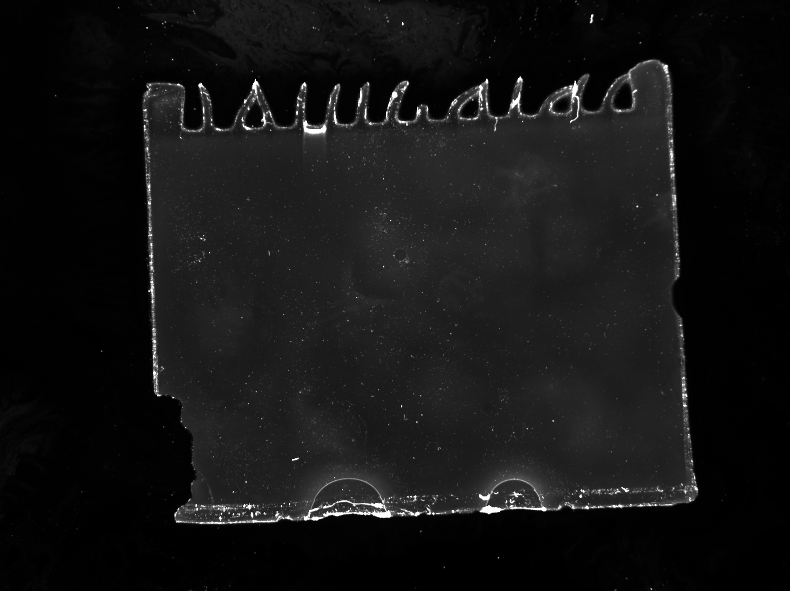
\includegraphics[width=0.3\textwidth]{./gels-old/40min-stain-40min-small.png}
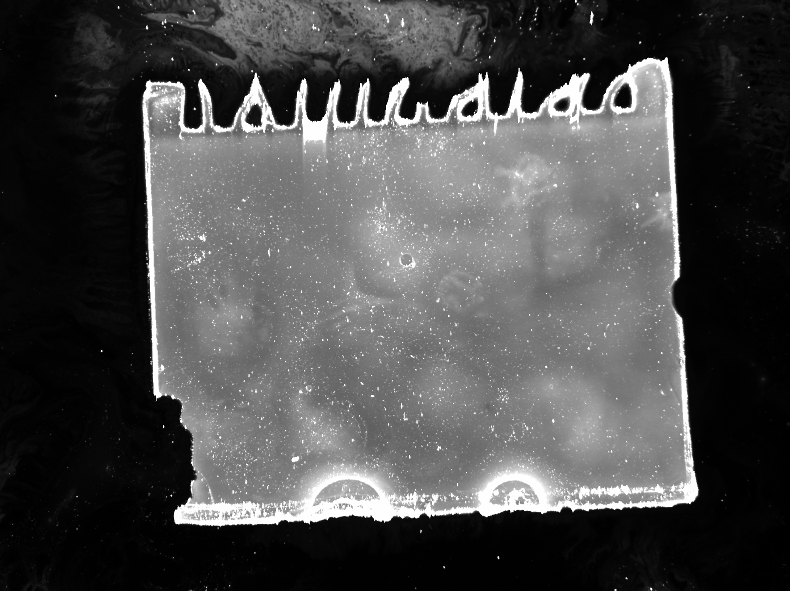
\includegraphics[width=0.3\textwidth]{./gels-old/overexpose-40min_stain-10sec-small.png}

\label{gels2}
\caption{Unedited Gels from Version 2}
Included for sake of completeness. This procedure did not succeed, likely because we did not remove the tape from our SDS-PAGE gel. Both gels have been stained for 40min, with the one on the left optimized for faint-bands and the one on the right overexposed for 10 seconds.
\end{center}
\end{figure}

\subsection{Procedure Notes}
None not already addressed. In summary, we should be more careful when pipetting samples into gels and we need to ensure that the buffer levels on our SDS-PAGE gels is sufficiently high.
\listoffigures
\bibliographystyle{ieeetr}
\bibliography{biblio}
\end{document}